% Header: Here are all packages used and some additional definitions
%%%%%%%%%%%%%%%%%%%%%%%%%%%%%%%%%%%%%%%%%%%%%%%%%%%%%%%%%%%%%%%%%%%

\documentclass[11pt,a4paper]{article}
\pdfminorversion=7
\usepackage[margin=2.5cm]{geometry}
\usepackage[onehalfspacing]{setspace}
\usepackage{graphicx} % zum Einbinden von Graphiken
\usepackage[breaklinks=true,colorlinks=true,linkcolor=blue,urlcolor=blue,citecolor=blue]{hyperref} % f. Referenzen
\usepackage{listings} % for code
\usepackage{amsmath,amsthm,amssymb} % Mathematik Umgebung 
\usepackage{icomma} % Intelligentes Komma, das den richtigen Abstand zwischen Dezimalzahlen als auch in Formeln wählt.
\usepackage[most]{tcolorbox}
\tcbset{promptstyle/.style={enhanced, boxrule=0.5pt, arc=2pt, fonttitle=\bfseries\sffamily\small, left=8pt, right=8pt, top=8pt, bottom=8pt}}
\usepackage[english]{babel} % Deutsche Bezeichnungen bei Inhaltsangabe etc
\usepackage[T1]{fontenc}    % andere Schriftsatzkodierung für richtige Silbentrennung bei Umlauten
\usepackage[locale = US, space-before-unit=true, per-mode=symbol]{siunitx} % Bessere Einheiten
\usepackage{placeins} % Definiert den Befehl “\FloatBarrier”, der die Ausgabe der davor eingebundenen Bilder erzwingt, befor der Text weiter geht. (Mit vorsicht zu verwenden)
\usepackage{float} % Provides [H] placement specifier for strict figure positioning
% \usepackage[natbib,abbreviate=true,doi=false,style=numeric-comp,giveninits=true,sorting=none]{biblatex} % Modernes Paket zur Erzeugung von Bibliografien (benötigt biber!)
\usepackage[utf8]{inputenc}
\usepackage{csquotes}
\usepackage[backend=biber]{biblatex}
\usepackage{svg}
\usepackage{amsmath} % usually needed if your SVG has text
\usepackage{booktabs}
\usepackage{tabularx}
\usepackage{caption}
\usepackage{pdflscape} % Key package for single-page landscape

\usepackage{xcolor}

% prompt stuff:
% Configuration for the JSON/Code blocks
\lstset{
    basicstyle=\ttfamily\scriptsize,
    breaklines=true,
    breakatwhitespace=true,
    columns=fullflexible,
    keepspaces=true,
    showstringspaces=false,
    literate={’}{{'}}1 {“}{{"}}1 {”}{{"}}1 % Fixes the UTF-8 Quote errors
}

% Reusable prompt style
\tcbset{
    promptstyle/.style={
        enhanced,
        boxrule=0.8pt,
        arc=3pt,
        fonttitle=\bfseries\sffamily\small,
        left=8pt, right=8pt, top=10pt, bottom=10pt,
        shadow={1mm}{-1mm}{0mm}{black!10}
    }
}


% for prompt diagram
% --- Design for the UI Boxes ---
\tcbset{
    promptstyle/.style={
        enhanced,
        boxrule=0.5pt,
        arc=2pt,
        fonttitle=\bfseries\sffamily\small,
        upper box=normal,
        left=8pt, right=8pt, top=8pt, bottom=8pt,
        toptitle=3pt, bottomtitle=3pt
    }
}

% Color definitions for better styling
\definecolor{barblue}{RGB}{51, 102, 204}
\definecolor{groupblue}{RGB}{51, 102, 204}
\definecolor{linkred}{RGB}{165, 0, 33}


\addbibresource{MyBibliography.bib} % Ort der .bib Datei, die die Datenbank für Literatur/Referenzen enthält.

\graphicspath{{Images/}}

\DeclareSIUnit{\dBm}{dBm}
\DeclareSIUnit[per-mode=reciprocal]\WN{\per\centi\meter}

%%%%%%%%%%%%%%%%%%%%%%%%%%%%%%%%%%%%%%%%%%%%%%%%%%%%%%%%%%%%%%%%%%%
\begin{document}
%
\title{\includegraphics[width=3.5cm]{logo.png} \\ \vspace{1cm} \textbf{Project Management Report}}
\author{Laura Kotalczyk \\ Manuel Mühlberger \\ \textbf{Group 4}}
\date{\today}
\maketitle
\vfill
\newpage
%
%
% \tableofcontents
\thispagestyle{empty}
\cleardoublepage
\pagenumbering{arabic} 
\newpage
%
%
\section{Project Vision and Scope}
\label{sec:project_vision}
%
\noindent
The vision of this project is to develop a more accurate and user-friendly mobile application for tracking daily nutritional intake by combining visual and spoken input through AI, addressing the common pain points of current calorie-tracking tools, such as time-consuming manual entry, limited context in meal logging as well as calorie underestimation by existing AI-enabled calorie trackers.

\noindent
Many users struggle to track self-cooked meals, mixed dishes, or food eaten outside the home (e.g., at restaurants or similar), because existing apps require users to manually search, estimate, or break down 
ingredients. Nowadays, some apps do leverage AI-enabled image recognition to streamline calorie tracking, promising greater ease and speed, however, these tools often fall short in accuracy, frequently over- or underestimating actual calorie count, which ultimately undermines the reliability of even the most convenient logging methods.
\\
To address this gap, our app introduces an additional input to the AI-enabled estimation approach: by simply taking a photo of a meal and adding a brief voice description, such as “pancakes with milk, no sugar, 3 eggs, 2 cups of flour, topped with some maple syrup”, users can instantly generate a more accurate estimate of calories and nutrients. By expanding the vision modality with contextual natural language input, the app harnesses modern AI technologies to deliver not just convenience, but more accurate, data-driven insights.
The goal is to reduce user effort and improve accuracy through its multi-modal approach, particularly for home-cooked and complex meals that are frequently misclassified or under-estimated in existing tools. The user can also browse a simple calendar view to display daily food intake and progress towards goals. Insights are provided to the user as well, so he can gain information on metrics such as average meal quality, longest logging streaks and many others.
\\
This solution aims to make nutrition tracking simpler, smarter, and more accessible, helping users stay aware of their intake and make informed choices, without requiring expertise meticulous manual logging.

\subsection{Key Deliverables and Defined Boundaries}

\subsubsection{Key Deliverables}

\noindent
\begin{minipage}{\textwidth}
    \centering
    \label{tab:deliverables}
    \small
    \begin{tabularx}{\textwidth}{l X}
        \toprule
        \textbf{Deliverable} & \textbf{Description} \\
        \midrule
        Mobile App Prototype & A basic app (Android/iOS) that lets users: take a photo of a meal and record a voice note (e.g., "pancakes with milk, no sugar, 3 eggs"). \\
        \addlinespace[10pt]
        Voice-to-Text Feature & The app automatically turns the voice description into text using an AI audio transcription model such as Whisper. \\
        \addlinespace[10pt]
        AI Nutrient Analyzer & Uses a Vision Language Model (VLM) (e.g., GPT-4V or Qwen-VL) to analyze the photo and text, and returns estimated calories and nutrients (e.g., "250 kcal, 12g protein"). \\
        \addlinespace[10pt]
        Central Server & Self-hosted Server taking care of input processing, forwarding, user authentication and data storage.  \\
        \addlinespace[10pt]
        Simple Dashboard & Shows daily calorie and nutrient intake in a calendar view. \\
        \addlinespace[10pt]
        Test Data \& Results & Uses 10–20 real example meals (e.g., homemade pancakes, homemade spaghetti Bolognese) with known nutrition values to test how accurate the app is. \\
        \addlinespace[10pt]
        Benchmarking Results & Uses the ground-truth real example meals for benchmarking the prototype against other competitor apps, evaluating its accuracy in estimation of nutrients and calories. \\
        \addlinespace[10pt]
        Project Report & A written report illustrating the design and functioning of the app, test results, and lessons learned from the project, in particular referring to the use of GenAI. \\
        \bottomrule
    \end{tabularx}
    \captionof{table}{Project Key Deliverables}

\end{minipage}

\subsubsection{Project Boundaries}
To keep the project focused and manageable, we decided on the following project boundaries as well as mandatory and optional app features.
\newline

\noindent
\textbf{In Scope}
\begin{itemize}
    \item User can record one photo and voice note per meal
    \item Use of open-source AI models for voice transcription and nutrient estimation (e.g., OpenAI API, Hugging Face, available ones on GitHub)
    \item Output includes estimated calories and macronutrients (carbs, protein, fat)
    \item Simple, modern and intuitive user interface
    \item Testing using 10–20 example meals with known nutritional values (manually calculated)
    \item User has the possibility to see real-time insights considering his meal tracking activities
    \item User can generate meal suggestions based on his current nutritional intake
\end{itemize}

\noindent
\textbf{Out of Scope}
\begin{itemize}
    \item Support for multiple languages or complex dishes with many unknown ingredients
    \item Integration with wearables or fitness trackers
    \item Integration of a user's training activities to increase available calories
    \item Nutrient database integration for more accurate results
    \item Possibility for data import/export
    \item Universally trusted server certificate
\end{itemize}

\section{Project Timeline \& Milestones}
\begin{figure}[htbp]
    \centering
    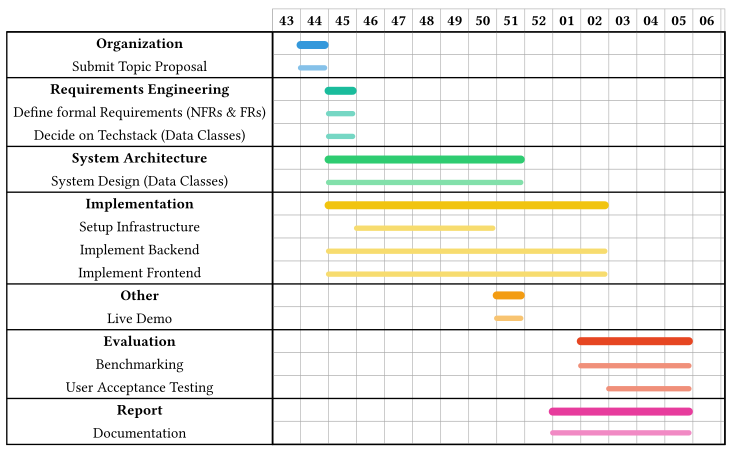
\includegraphics[width=0.9\textwidth]{gantt.png}
    \caption{Project Timeline and Milestones}
\end{figure}

\section{System Architecture and Technical Design}

\subsection{High-Level System Design}
\noindent
With respect to system design, we decided on a server-client architecture, involving two locally hosted servers and one externally hosted proxy server.
First and foremost, the NutriAI server (1) serves as the central communication hub, orchestrating all internal and external data flows. It manages and routes interactions between clients, the database, and external APIs, handling critical functions such as user sign-up, authentication, rate limiting, and database operations, ensuring seamless and secure system performance. \\
Secondly, server two (2) runs a reimplementation of OpenAI's Whisper model \cite{whisper}, that is used for transcribing a user's recorded voice note in the AI-assisted meal logging workflow. \\ Thirdly, the proxy server (3) handles the connectivity between the server and the clients. It acts as a load balancer \cite{pangolin, traefik} and a firewall that blocks malicious actors from reaching the server \cite{pangolin, crowdsec}. The client connects to the server domain, which points to the proxy server, forwarding all requests to the main NutriAI server. A more in-depth technical explanation is given in chapter \ref{chap:3.2}.

\begin{figure}[htbp]
    \centering
    \includesvg[width=0.9\textwidth]{system_design.svg}
    \caption{High-Level System Architecture of NutriAI}
    \label{fig:system_design}
\end{figure}

\noindent
By hosting all user data on our own locally managed server, we eliminate reliance on external service providers for storing sensitive information, allowing us to maintain a better control over the data. Furthermore, our locally hosted implementation of OpenAI’s Whisper model ensures that user voice data is never shared with external systems or used for AI training. Instead, audio recordings are securely processed within our private infrastructure, and only the resulting transcription, paired with the user’s meal photo, is sent to the externally hosted VLM. A more detailed explanation on data privacy and possible improvements in this regard for our service is given in the Project Safety and Reflection Report.
\FloatBarrier\subsection{Core Technical Components}
\label{chap:3.2}
In the following paragraphs, we will elaborate on each of our system's components from a technical perspective, pointing out its role and interactions in the overall system.

\subsubsection{Client}
\noindent
Since we were aiming at building a mobile app that runs cross-platform, we opted for Expo (version 54), after some research on possible options. Expo is a full-stack React Native framework that offers a rich ecosystem of pre-built components and tools, known for its simple setup, fast prototyping, and smooth development workflow \cite{expo}. Its accessibility made it a strong fit for our team, particularly given the varying levels of experience among team members. Thus, the client can either be an iOS or Android user. In the current development build, the app requires the user to have a custom certificate installed on their device, for encrypted communication with the NutriAI server. This limitation is due to time constraints, and for a production build it would be possible to host a universally trusted Let's Encrypt certificate on the server \cite{lets}.\\
The client does not manage a conventional database itself, but rather only has a minimal key-value store (react-native-async-storage) \cite{async} functioning as a caching layer. Here, frequently accessed data like the user profile, recent meal data (pictures, nutrients), etc. are stored. This enables the app to have a partially functional offline mode, where the user can still interact, although with limited functionality. 

\subsubsection{Proxy}
When the user uses the app to sign up, login or log a meal, corresponding requests are sent to the proxy server.
 This server is hosted as a docker stack on a Virtual Private Server (VPS) supplied by a Cloud Provider (Hetzner). It comprises of two main parts: Traefik and CrowdSec and the main Pangolin server. \\
 The NutriAI domain points directly to Traefik, which acts as the initial entry point for all incoming application traffic on the VPS. Traefik serves as a reverse proxy and load balancer, utilizing a specific middleware integration with CrowdSec to identify and block malicious requests before they reach the backend.
 Pangolin manages the "allowed" request flow by utilizing Newt, a user-space WireGuard tunnel client, to securely forward traffic to the on-premise server. This distributed architecture shields the internal infrastructure from malicious actors by punching through NAT and firewall restrictions without requiring open inbound ports. Furthermore, this setup facilitates high availability and failover, as a single Pangolin instance can coordinate and route traffic across multiple Newt site connectors.


\subsubsection{Server}
The On-Premise Server operates as a composed Docker stack on a shared Docker network, consisting of three primary components: the Newt connector, the Whisper transcription service, and the main NutriAI executable. As detailed in the Proxy section, the Newt container maintains the secure WireGuard tunnel, receiving forwarded requests from the upstream Pangolin instance and returning Nutri AI server responses. For voice processing, the system utilizes faster-whisper; however, to mitigate the lack of security in the stock container, a custom wrapper was implemented to handle authentication via API keys.
\\
The core NutriAI server handles the main application logic, utilizing the aforementioned custom SSL certificate for encrypted communication to the clients and an SQLite database for persistent storage. User credentials are secured using bcrypt to salt and hash passwords, and successful login or sign-up events issue a JSON Web Token (JWT) to authenticate subsequent requests. When processing a meal log, the server forwards the audio (.wav) file internally to Whisper, then combines the resulting transcription with the user’s image and a system prompt to send to an external OpenAI-compatible VLM endpoint. This design enables flexibility in model selection. While locally hosting the VLM would be an ideal feature to keep all data on-premise and the open source selection of VLM's is great, hardware constraints necessitated an external solution for this project. The server parses the VLM's structured JSON response — containing the meal name, description, and nutritional info — and stores it alongside the media in the database for the client to retrieve.

\section{Methodology}

\subsection{Project Management}
To organize our team and the development process of the mobile application properly, we decided on a ''SCRUM-alike'' agile work mode. We proceeded in increments of one-week long sprints, agreeing on tasks each of the team members should finish until the next week. During our weekly meeting slot in person, we then met to discuss our progress on the respective tasks, next steps and potential impediments. Apart from that, we added new items and bug fix tickets to the product backlog, prioritized the product backlog and assigned tasks with respective deadlines to team members.
\begin{figure}[htbp]
    \begin{center}
    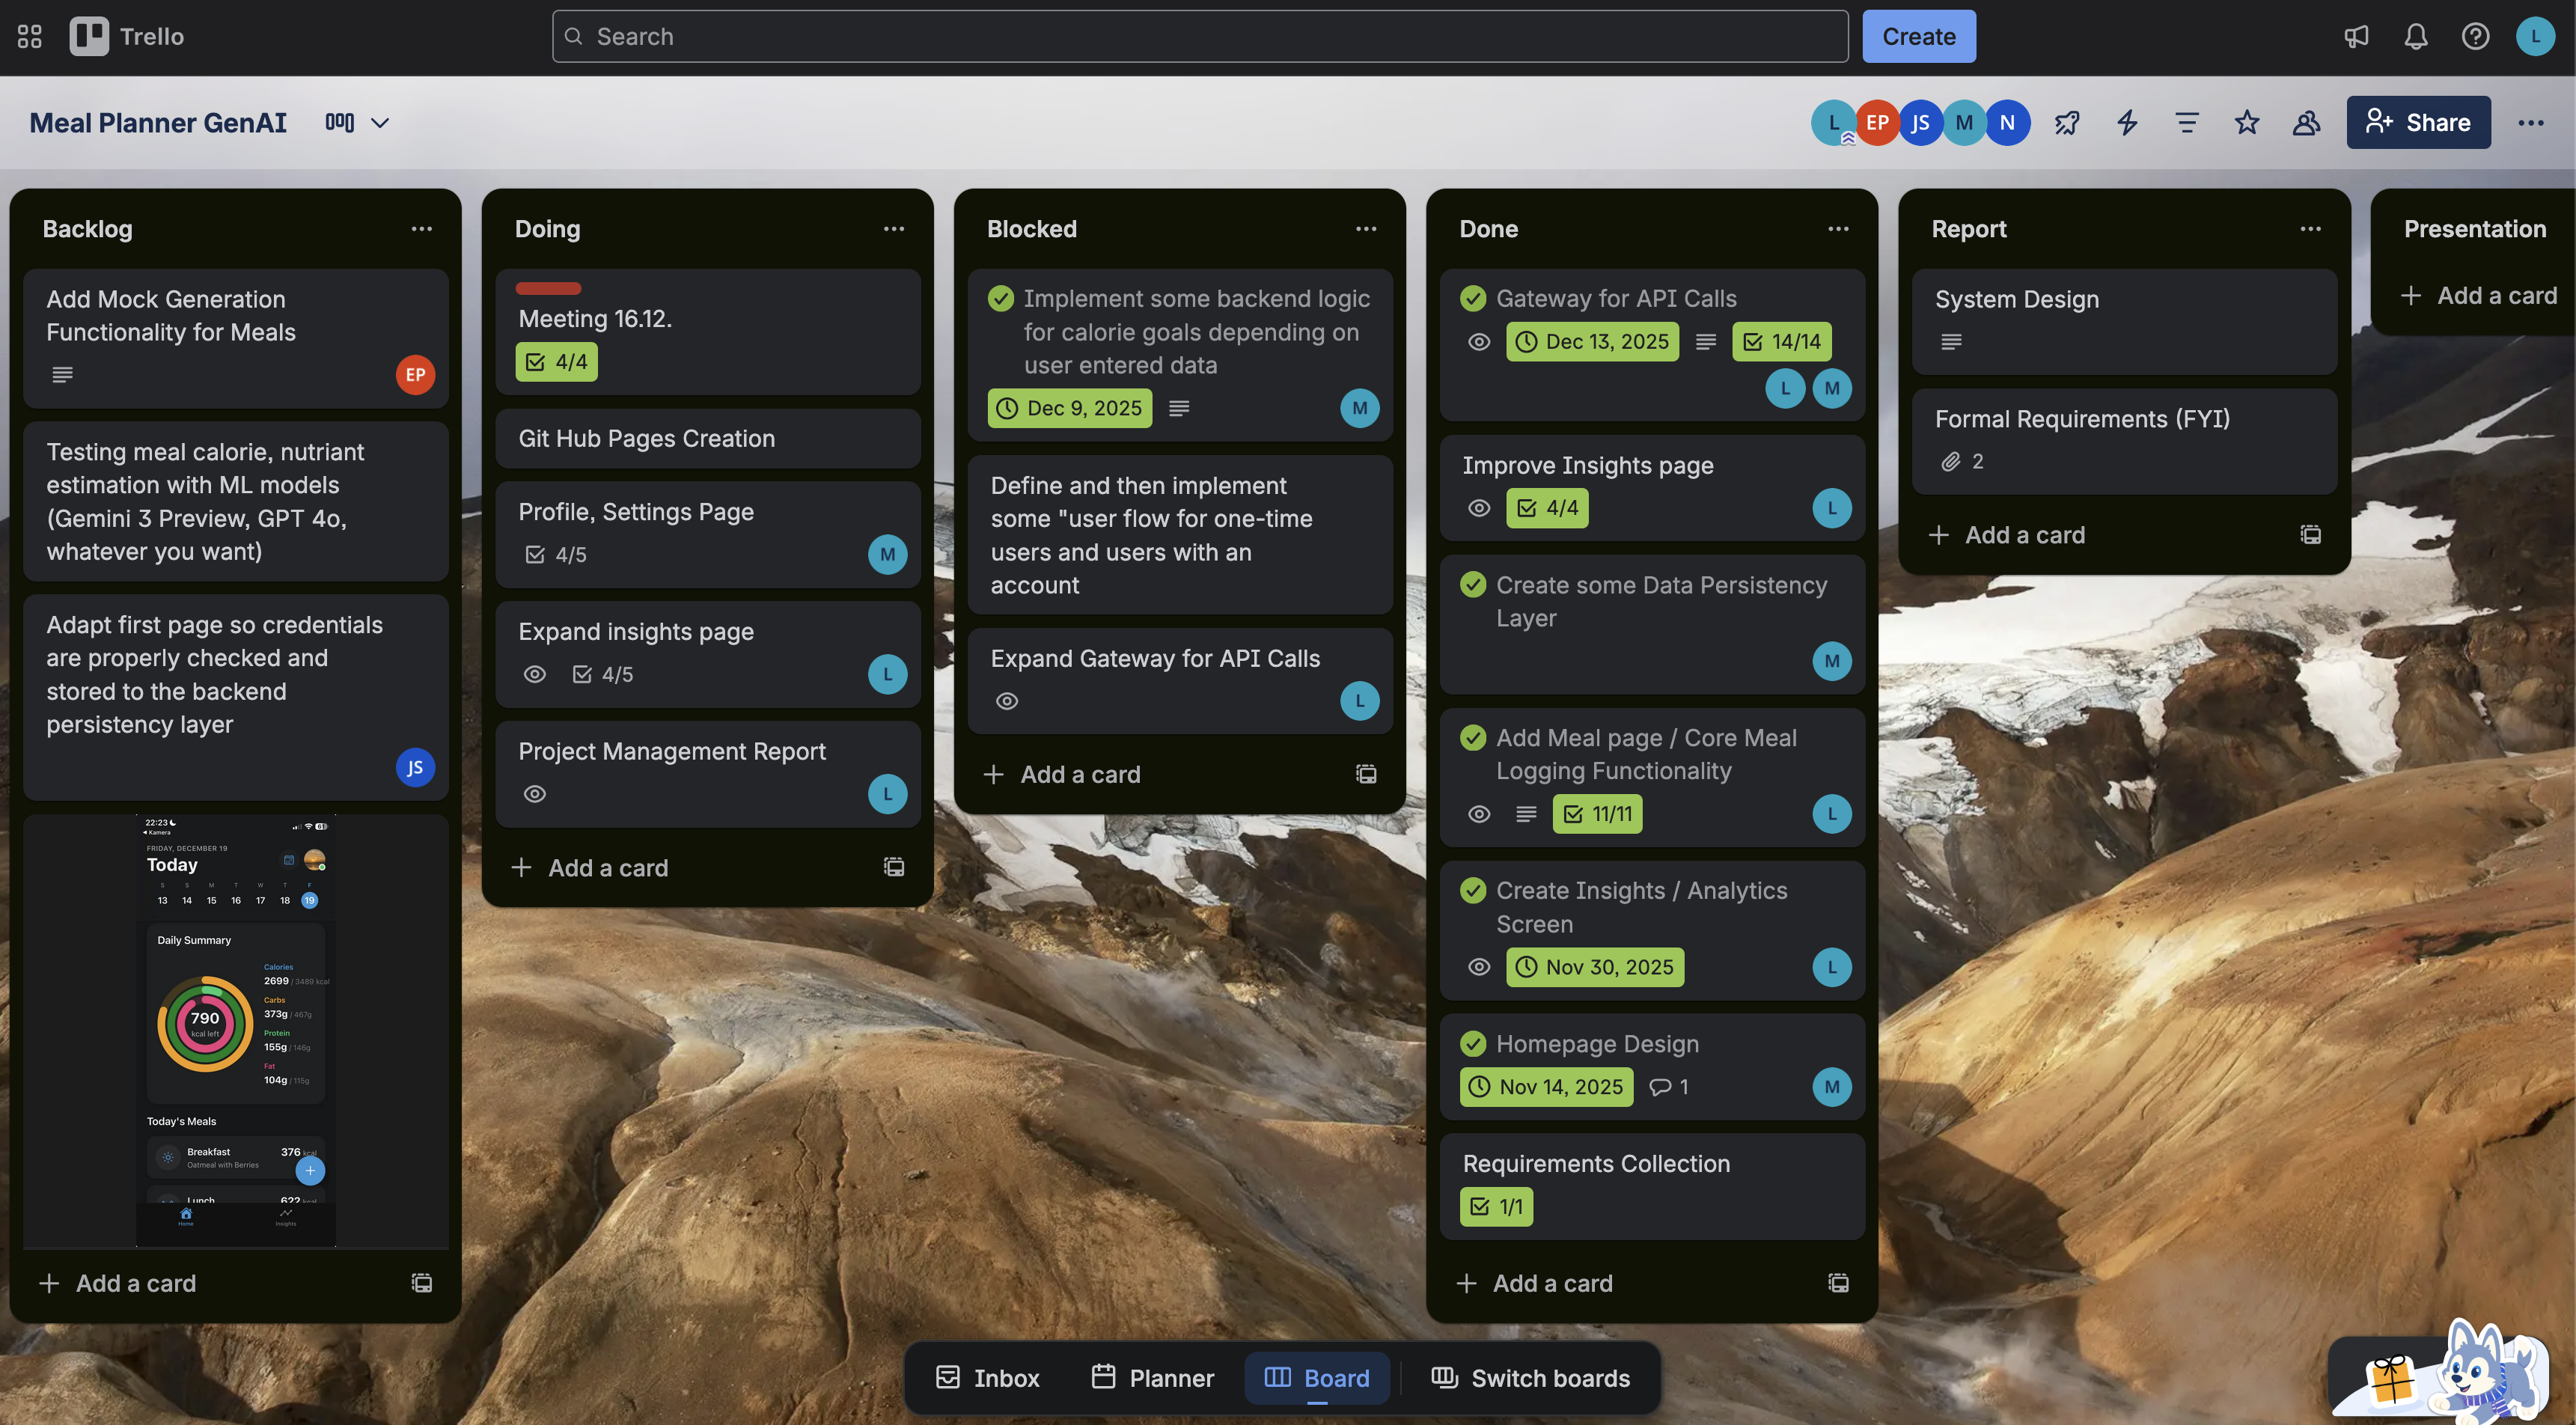
\includegraphics[width=0.8\textwidth]{trello.png}
    \caption{Project Management Board used for Development of NutriAI}
    \label{fig:trello}
    \end{center}
\end{figure}

\noindent
To keep track of the tickets and overall tasks concerning our project, we used Trello, a project management tool that uses a flexible, Kanban-style system of boards, lists, and cards to help individuals and teams organize tasks, workflows, and ideas, making it easy to track progress from "to-do" to "done" \cite{trello}. For a screenshot taken from our project's board, refer to Figure \ref{fig:trello}.
Apart from using a project management tool, we also created a WhatsApp group with all the team members to agree on meeting dates, keep us updated and discuss immediate questions or provide advice quicklier.
\\
With respect to roadmap planning, our overall strategy, in terms of application design, was to go from the coarse overview to the more granular subsystems, and, thereby, develop in a step-by-step fashion. We started with a target audience analysis to inform and guide the requirements engineering process, resulting in the functional (FRs) and non-functional (NFRs) requirements our application needed to meet. Following our requirements collection, we then proceeded with system design. Once an initial architecture was established, we began with the implementation, making adjustments as needed to accommodate changes or unforeseen challenges. A more detailed explanation for our techniques employed during system design as well as database design will be given in sections \ref{chap:sys} and \ref{chap:db}, respectively. After completing the overall implementation, we initiated user acceptance testing to gather feedback on the application and identify any remaining weaknesses or areas needing improvement. Based on the feedback from user acceptance testing, we then focused on addressing the identified areas to enhance usability, and overall quality.

\FloatBarrier
\subsection{System Design}
\label{chap:sys}
The system design was informed by a set of functional and non-functional requirements collected early in the project. Since our target audience includes both iOS and Android users, a cross-platform solution was required, which led us to choose React Native together with Expo. On the backend, a key requirement was centralized user account management and a single, controlled access point for all AI API calls. Routing these requests exclusively through the server allows us to handle the requirements of authentication, rate limiting, and API key management centrally, without exposing sensitive logic or credentials to the client.
\\
Another important consideration was the intended deployment model. From the beginning, the system was designed to run on an on-premise server, complemented by a manually managed VPS that serves as an external access point. This setup motivated the use of Docker, as containerization ensures that all services remain isolated, reproducible, and easy to operate across both environments. In addition, this approach allows future extensions such as scaling or failover to be implemented with relatively little effort. Together, these requirements naturally led to a clear server--client separation and the use of a reverse proxy pattern, which provides a well-defined boundary between mobile clients and the internal infrastructure.
 
\subsection{Database Design}
\label{chap:db}
Based on the collected requirements, we identified four core data classes for the application: \textit{User}, \textit{MealEntry}, \textit{NutritionInfo}, and \textit{Day}. The \textit{User} entity stores basic profile information (e.g., name, age, and weight), health-related data such as medical conditions and personal goals, as well as authentication data in the form of an email address and a hashed password. Each \textit{MealEntry} represents a logged meal and contains a timestamp, a meal category, optional references to an image and a transcription, and an associated \textit{NutritionInfo} object holding estimated macronutrients. A meal quality score is derived from factors such as calorie density and goal alignment. The \textit{Day} entity groups all meals of a specific date and stores target nutrition values to enable daily comparisons.
\\
During early development, we used simple JSON-based storage to iterate quickly on the data model. As the system evolved and requirements such as multi-user support, structured queries for calendar views, and data consistency became more important, we migrated to SQLite. A practical advantage of SQLite in this context was its flexibility, as schema changes (e.g., adding new columns) could be applied with minimal overhead, while still providing reliable relational storage. At the same time, SQLite remains lightweight and well suited for deployment within our Docker-based backend, without the complexity of operating a separate database server.

\FloatBarrier
\subsection{Prompt Engineering}
During the development process, we applied various prompt engineering techniques to evaluate and compare two distinct prompt sets for our main feature - one simpler and one more complex. The prompt set includes the system and user prompt. 
For the first prompt set, we devised a straightforward task description, providing the model with minimal context. This included a basic ruleset and an example JSON template to guide the model’s output, specifically designed for our desired meal analyzer use case. \\
\noindent
For the second prompt set, we utilized various prompt engineering techniques presented in the lecture.
Adopting a meta-prompting approach, we used Google’s Gemini 3 Flash Preview model to generate a suitable prompt for our use case. We began by providing it with a foundational context for the task, then explicitly instructed it to adopt the persona of a prompt engineer. We asked it to analyze the requirements and clearly articulate exactly what information it needed to craft an effective, targeted, and well-structured prompt. In addition, we instructed the model to request further context or clarification if any ambiguity or imprecision remained, and to explicitly signal when the prompt had reached a sufficiently accurate state, ensuring we could collaboratively finalize it confidently. Following our initial prompt, the model requested clarification, particularly regarding which input to prioritize in cases of ambiguity between image and text/transcription. After addressing these unclear aspects, we received a precise and sophisticated system prompt, along with a rather simple user prompt. We opted for a structured prompt, used delimiters to clearly indicate distinct parts of input and specifically stated our desired output format, a custom JSON. Additionally, during the development of prompt set two, we incorporated a full example, comprising an image and its corresponding transcription, to guide and inform prompt design. For both prompt sets, we also provided an example output to facilitate in-context learning.\\
\noindent
With these two versions, we now proceeded evaluating and comparing the performance of both prompt sets with different models and a set of ground truth meals\footnote{Ground truth meals are those for which we have both an image and complete nutritional data, enabling us to accurately assess and compare the performance of different prompt sets.}.
\\
\noindent
Against all expectations, the simpler prompt set performed much better in meal calorie and nutriant estimation than the second, more detailed prompt set.
Although both prompt sets, across all tested models, were overestimating calorie and nutriant values, prompt set one was still the more precise one of the two. Consequently, we kept prompt set one as our production-level prompt set.
On a smaller set of ground truth meals, we also assessed whether varying temperatures changed the estimation quality. This, however, was not the case; results were neither less precise nor more accurate, so we decided to leave the selected temperature at 0.0.
As we observed that the model consistently overestimated fat values and miscalculated portion sizes, we further refined the production prompt. We added a specific instruction to maintain conservative estimates, directing the model to assume standard restaurant portions of approximately 100-150g for proteins, and to assign high fat or carbohydrate values only when visual evidence of oil, frying, or large starch portions was clearly present.
\\
Finally, a comprehensive VLM evaluation against our ground truth meal dataset, revealed that among all tested models, \texttt{qwen3-vl-235b-a22b-instruct} was the most precise in nutrient estimation, serving as our current production-ready model.

\FloatBarrier
\section{Team roles}

\noindent
The NutriAI project team comprised five members with overlapping responsibilities across key development phases. Laura and Manuel shared the product owner role, guiding feature prioritization, while also serving as architects who defined and implemented the system's technical structure. In implementation, Manuel, Laura, and Eduardo worked as full-stack developers, while Joana focused on the frontend task that is the first-time user setup. Manuel managed deployment and operations. For evaluation and testing, Joana conducted user acceptance testing, authoring the corresponding report, and performed market research comparing competitor apps to the NutriAI product. Laura performed prompt and VLM evaluations by using a self-developed dataset, and Eduardo created the user guide. In other roles, Laura and Manuel co-authored the project management and safety reports, while Nils developed the presentation slides and served as the point of contact for repository administration.

\begin{figure}[htbp]
    \centering 
    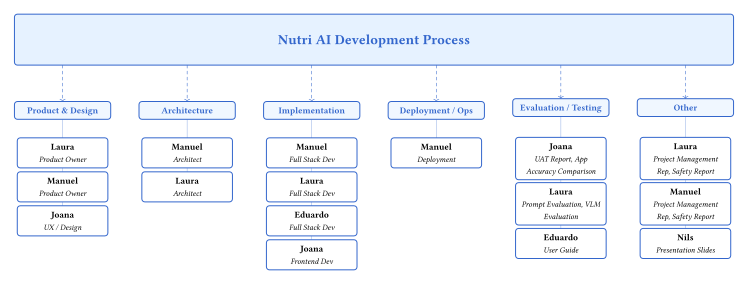
\includegraphics[width=0.9\textwidth]{typst_plots_out/org_chart.pdf}
    \caption{Team Chart}
\end{figure}
 
\section{Evaluation}
\label{chap:eval}
\noindent
The evaluation results, as shown in Table \ref{tab:mean_percentage_error} and Figures \ref{fig:overall_mae_bar} and \ref{fig:percentage_error_boxplots}, provide a detailed comparison of the performance of NutriAI and other applications in nutrient estimation. The Mean Percentage Error (MPE) table indicates that NutriAI with both photo and audio inputs achieves relatively strong accuracy across all nutrients. For example, in the carbohydrate category, the MPE decreases from 45.70\% (photo-only) to 38.21\% when audio input is included. This suggests that the additional context from voice descriptions can help the model better interpret certain types of meals, particularly those that are more complex or ambiguous.

\begin{table}[H]
\centering
\begin{tabular}{l r r r r}
\toprule
\textbf{App} & \textbf{Calories} & \textbf{Carbs} & \textbf{Proteins} & \textbf{Fats} \\
 & \textbf{MPE (\%)} & \textbf{MPE (\%)} & \textbf{MPE (\%)} & \textbf{MPE (\%)} \\
\midrule
NutriAI: Photo Input only & 20.62 & 45.70 & 16.42 & 14.11 \\
NutriAI: Photo + Audio Input & 21.96 & 38.21 & 18.60 & 44.60 \\
CalorieCueAI & 41.06 & 45.89 & 40.16 & 78.17 \\
CalorixAI & 25.09 & 18.90 & 27.83 & 97.66 \\
arise & 46.22 & 32.78 & 65.83 & 147.91 \\
\bottomrule
\end{tabular}
\caption{Mean Percentage Error (MPE) by App and Nutrient. The MPE is calculated as $(Estimation - Ground Truth) / Ground Truth \times 100$. Positive values indicate overestimation, while negative values indicate underestimation of the actual nutritional content.}
\label{tab:mean_percentage_error}
\end{table}

\noindent
The bar chart in Figure \ref{fig:overall_mae_bar} shows that NutriAI with audio input performs well in terms of overall Mean Absolute Percentage Error (MAPE) compared to the other tested applications. This metric was chosen to provide a general view of performance by aggregating errors across all nutrients, offering a useful perspective on overall accuracy.

\begin{figure}[htbp]
\centering
\includegraphics[width=0.9\textwidth]{typst_plots_out/overall_mae_bar.pdf}
\caption{Overall Mean Absolute Percentage Error by App.}
\label{fig:overall_mae_bar}
\end{figure}
\noindent
The boxplots in Figure \ref{fig:percentage_error_boxplots} highlight the variability in performance across different apps and nutrients. NutriAI's results, particularly with audio input, show a narrower interquartile range (IQR) for some nutrients, indicating more consistent estimations. However, the results also reveal areas for improvement, such as increased variability in fat estimation when audio input is included. This suggests that while audio input generally contributes to better accuracy, it may also introduce some inconsistencies in specific cases, pointing to the need for further refinement in the integration of multi-modal data.

\begin{figure}[htbp]
\centering
\includegraphics[width=0.95\textwidth]{typst_plots_out/percentage_error_boxplots.pdf}
\caption{Distribution of percentage errors across all apps and nutrients. Each box represents the interquartile range (IQR) with the median shown as a line inside the box. Whiskers extend to the minimum and maximum values. The dashed horizontal line at 0\% represents perfect accuracy. Values above 0\% indicate overestimation, while values below 0\% indicate underestimation.}
\label{fig:percentage_error_boxplots}
\end{figure}

\noindent
By using both MPE and MAPE, the evaluation provides a balanced understanding of the models' performance. MPE is effective for assessing individual nutrient estimations, while MAPE offers a broader measure of overall accuracy, ensuring a comprehensive analysis.
\section{Current Progress and Future Plans}
As of today, our nutrient estimation service has made significant progress in achieving its core objectives. The application now enables users to log their meals by capturing a photo and recording a voice note, allowing for AI-enabled nutrient and calorie estimation. This multi-modal approach ensures greater accuracy, particularly for complex or home-cooked meals. Additionally, the app provides meal suggestions tailored to the user’s past caloric and nutrient intake, helping them make informed dietary choices. Furthermore, the app offers analytics and insights, such as average meal quality, daily food intake, progress towards goals, and logging streaks, empowering users to better understand and manage their nutrition. While these features form the foundation of our service, there remain several areas for optimization prior to a full production rollout:

\begin{itemize}
    \item \textbf{Re-Prompting}: Currently, while users can manually adjust nutrient values and descriptions, the system lacks the capability to trigger a new VLM inference based on those corrections. Implementing a re-prompting mechanism, for instance, allowing the model to correct a misidentification of falafel as meatballs, would likely yield more precise results and streamline the user experience by preventing manual data entry.
    \item \textbf{Inference Latency}: Although the  \texttt{qwen3-vl-235b-a22b-instruct} model delivers high precision, its current processing time is a bottleneck for real-time application usage. Reducing this latency is a critical requirement for ensuring a convenient and fluid user interface.
    \item \textbf{UI/UX Refinements}: As detailed in our UAT report, several design improvements are necessary to increase intuitiveness. Specifically, interactive elements, such as the highlights in the 'Insights' tab, require clearer visual affordances to indicate they are clickable, as their current design does not effectively communicate their underlying functionality.
    \item \textbf{Traditional Logging Features}: Beyond AI-driven estimation, integrating traditional logging methods, such as barcode scanning and verified nutrient database queries, would provide a more comprehensive and accurate baseline for user data and would give the user more flexibility.
    \item \textbf{Out of Scope Features}: Apart from the more technical flaws our service could improve on, future steps could also include adding other features that were out of scope for the project timeline so far, such as a possibility for data im- and export or multi-language support.
\end{itemize}
\noindent
There remain several avenues to improve the app’s stability and performance. Specifically, the AI framework allows for ongoing optimization through larger-scale ground truth testing, alternative prompting methodologies, and the continuous evaluation of emerging architectural models.

\section{Project Pitch Video (Attached)}

\section{Usage of GenAI during the Document's Creation}
\noindent
Generative AI was used during the writing process to help with brainstorming and organizing initial notes, and rephrasing passages.
It was also used to assist with debugging problems occuring with LaTeX.


\printbibliography

\end{document}
